\documentclass[11pt]{article}

\usepackage[margin=1in]{geometry}
\usepackage[T1]{fontenc}
\usepackage[utf8]{inputenc}
\usepackage{lmodern}
\usepackage{microtype}
\usepackage{graphicx}
\usepackage{booktabs}
\usepackage{tabularx}
\usepackage{array}
\usepackage{amsmath}
\usepackage{caption}
\usepackage{enumitem}
\usepackage{xcolor}
\usepackage[section]{placeins}
\usepackage[hidelinks]{hyperref}

\captionsetup{font=small,labelfont=bf}
\setlist{itemsep=2pt,topsep=4pt}
\newcolumntype{L}{>{\raggedright\arraybackslash}X}
\newcolumntype{R}{>{\raggedleft\arraybackslash}r}

\title{Benchmarking Compact Convolutional Transformers\\using the BigEarthNet Dataset}
\author{William Gullett}
\date{Revised November 2026\thanks{This is a corrected and extended version of a Major Research Project
submitted to Toronto Metropolitan University in 2024 for the M.Sc.\ in Data Science and Analytics.
Section~\ref{sec:revisit} explains what changed and why.}}

\begin{document}
\maketitle

\begin{abstract}
\noindent
Land use and land cover (LULC) classification needs models that are accurate but cheap to train.
Compact Convolutional Transformers (CCTs) were designed for exactly that trade-off, yet they have not been
benchmarked on BigEarthNet, the standard large-scale multi-label LULC dataset. An earlier version of this
study reported that CCT-2 and CCT-4 reached a micro-F1 of only about 18\% and concluded that CCTs were not
viable. This revision shows that those figures came from an evaluation error in which predictions were
scored against the labels of different images, and it repeats the benchmark with a corrected pipeline.
A CCT-7 with 3.94 million parameters, trained from scratch on the RGB rendering of BigEarthNet-19 for
30 epochs, reaches a test micro-F1 of 78.4\% (precision 80.8\%, recall 76.1\%), a macro-F1 of 72.4\% and a
mean average precision of 79.5\%. Training took 38.5 minutes on one NVIDIA A100 GPU. These scores fall in
the range reported for the 60 models benchmarked by Papoutsis et al.~\cite{papoutsis}, although that
comparison is indicative only, because those models were trained on multispectral input and a larger patch
set. The results reverse the earlier conclusion: a small CCT is both accurate and inexpensive on this task.

\medskip
\noindent\textbf{Keywords:} compact convolutional transformers, land use and land cover, BigEarthNet,
multi-label image classification, remote sensing
\end{abstract}

%------------------------------------------------------------------------------
\section{Introduction}

Land use and land cover classification assigns to each satellite image the kinds of surface it contains,
such as forest, arable land, urban fabric or water. It supports urban planning, wildfire detection,
surface-temperature studies and forest monitoring, and it depends on models that can be trained and run
at reasonable cost.

Compact Convolutional Transformers~\cite{hassani} pair a small convolutional tokenizer with a transformer
encoder. They were designed to work on small datasets and with few parameters, and their authors showed
that the design scales: CCT-14 reaches 80.67\% top-1 accuracy on ImageNet. CCTs have also done well on
other satellite-imagery tasks, including landslide susceptibility mapping~\cite{zhao} and hurricane damage
identification~\cite{islam}. They had not, however, been benchmarked on BigEarthNet.

This study asks whether CCTs are a viable model family for multi-label LULC classification on
BigEarthNet, and how their accuracy and training cost compare with the models benchmarked by Papoutsis
et al.~\cite{papoutsis}. It makes three contributions:

\begin{enumerate}
  \item A corrected benchmark of CCT-7 on BigEarthNet-19, with a test micro-F1 of 78.4\% from a
        3.94-million-parameter model trained in under 40 minutes.
  \item A diagnosis of why the 2024 version of this study reported a micro-F1 near 18\%, including a
        control experiment that reproduces the faulty evaluation on a working model.
  \item An openly available training and evaluation pipeline for BigEarthNet RGB data that runs in a
        single Google Colab session.
\end{enumerate}

%------------------------------------------------------------------------------
\section{Literature Review}

\paragraph{Uses of LULC classification.}
Bokhari et al.\ used classification and regression trees to track regulated and semi-regulated urban
development~\cite{bokhari}. Urbanelli et al.\ combined classical machine learning with ResNets in a
multimodal approach to wildfire identification~\cite{urbanelli}. Choudhary and Ramkumar reviewed
AI methods for measuring the spread of an invasive tree species from satellite images~\cite{choudhary}.
Kim, Kim and Kim used explainable AI to relate LULC to land surface temperature~\cite{kim}. Vincent et
al.\ detected LULC change in several Indian districts to measure city growth~\cite{vincent}. Shaik et al.\
classified canopy height, tree species and LULC to study forest temperature dynamics~\cite{shaik}, and
Mannan et al.\ used LULC change to monitor forest loss in Pakistan~\cite{mannan}.

\paragraph{Deep learning for LULC.}
Naushad et al.\ compared several CNNs and classical methods on EuroSAT and found ResNet-50 the most
accurate at 99.17\%~\cite{naushad}. Jamali et al.\ proposed SGU-MLP, an MLP-based model for settings with
few training examples, and reported the best average accuracy among the CNN and CNN--ViT models they
tested~\cite{jamali}. Kunwar and Ferdush compared ResNet-50, ViT and VGG16 on EuroSAT and found the
Vision Transformer the most accurate at 99.19\%~\cite{kunwar}. Neither convolutional nor transformer models
have a settled advantage, which makes a hybrid of the two worth testing.

\paragraph{The BigEarthNet benchmark.}
Papoutsis et al.~\cite{papoutsis} benchmarked more than 60 models on BigEarthNet, covering ResNets,
DenseNets, VGG, EfficientNets, Wide Residual Networks, Vision Transformers and MLP-Mixers. All were
trained from scratch for 30 epochs with binary cross-entropy. Their best model by F-score, a Wide Residual
Network with efficient channel attention, reaches 79.0\%. That study is the reference point here.

\paragraph{Compact Convolutional Transformers.}
Hassani et al.~\cite{hassani} introduced CCTs to reduce the reliance of transformers on very large
datasets. A CCT replaces the patch embedding of a Vision Transformer with a few convolution and pooling
layers, which preserves local structure and gives richer tokens, and replaces the class token with a
learned weighted average over all tokens (sequence pooling). Zhao, Chen and Li found that a CCT
outperformed ViT, ResNet and a plain CNN for landslide susceptibility mapping~\cite{zhao}, and Islam et
al.\ found that it outperformed VGG16, ResNet-50, Inception-V3 and AlexNet at identifying hurricane damage
in satellite images~\cite{islam}.

%------------------------------------------------------------------------------
\section{Dataset}

BigEarthNet~\cite{sumbul} was built by the Remote Sensing Image Analysis group and the Database Systems
and Information Management group at TU Berlin. BigEarthNet-S2 version~1 contains 590,326 Sentinel-2
patches acquired over ten European countries in 2017 and 2018. Each patch is $120\times120$ pixels at
10\,m resolution, covering 1.2\,km $\times$ 1.2\,km, and carries one or more CORINE Land Cover labels.
Version~1 is used so that results can be set beside those of~\cite{papoutsis}.

\paragraph{Copy used.}
This study uses the copy hosted on the Hugging Face Hub under the name
\path{danielz01/BigEarthNet-S2-v1.0}. It provides each patch as an 8-bit RGB image and excludes the
patches covered by seasonal snow, cloud or cloud shadow, as the dataset authors recommend. It has
519,284 patches in the predefined splits shown in Table~\ref{tab:splits}. The RGB images are dark: the
mean pixel value in the training split is 14.9 on a 0--255 scale, with a standard deviation of about 44.
Inputs are therefore standardised per channel with statistics from the training split.

\begin{table}[!htbp]
\centering
\caption{Dataset splits. Every patch retains at least one label after conversion to 19 classes.}
\label{tab:splits}
\begin{tabular}{lrrr}
\toprule
Split & Patches & Share & Labels per patch \\
\midrule
Training   & 269,695 & 51.9\% & 2.90 \\
Validation & 123,723 & 23.8\% & 2.89 \\
Test       & 125,866 & 24.2\% & 2.88 \\
\midrule
Total      & 519,284 & & \\
\bottomrule
\end{tabular}
\end{table}

\paragraph{Labels.}
The 43 original classes are converted to the 19-class nomenclature used in~\cite{papoutsis}:

\begin{itemize}
  \item \emph{Urban fabric}: continuous and discontinuous urban fabric.
  \item \emph{Arable land}: non-irrigated arable land, permanently irrigated land, rice fields.
  \item \emph{Permanent crops}: vineyards, fruit trees and berry plantations, olive groves, annual crops
        associated with permanent crops.
  \item \emph{Natural grassland and sparsely vegetated areas}: natural grassland, sparsely vegetated areas.
  \item \emph{Moors, heathland and sclerophyllous vegetation}: moors and heathland, sclerophyllous vegetation.
  \item \emph{Inland wetlands}: inland marshes, peatbogs.
  \item \emph{Coastal wetlands}: salt marshes, salines.
  \item \emph{Inland waters}: water courses, water bodies.
  \item \emph{Marine waters}: coastal lagoons, estuaries, sea and ocean.
  \item Eleven classes are removed: road and rail networks, sport and leisure facilities, port areas,
        airports, mineral extraction sites, dump sites, construction sites, green urban areas, bare rock,
        burnt areas and intertidal flats.
\end{itemize}

The remaining classes are kept unchanged. The task is multi-label: a patch averages 2.9 labels.

\paragraph{Class imbalance.}
The classes are far from balanced (Figure~\ref{fig:balance}). In the training split, \emph{Arable land}
appears in 37.2\% of patches and \emph{Coastal wetlands} in 0.4\%, a ratio of 97 to 1. Six classes each
appear in fewer than 5\% of patches. Imbalance of this size is the reason the evaluation reports
class-averaged metrics beside the micro-averaged ones.

\begin{figure}[!htbp]
\centering
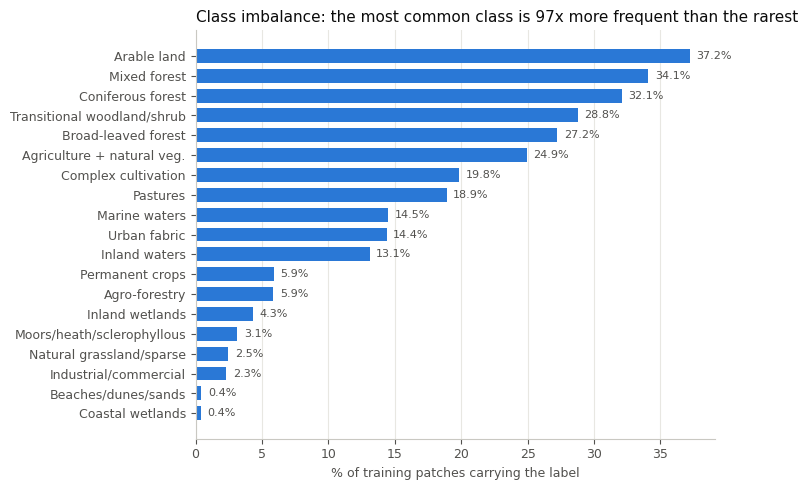
\includegraphics[width=0.78\linewidth]{figures/class_balance.png}
\caption{Share of training patches carrying each of the 19 labels.}
\label{fig:balance}
\end{figure}

%------------------------------------------------------------------------------
\section{Methodology}

\subsection{Model}

The model is CCT-7 as defined in~\cite{hassani}: seven pre-norm transformer encoder layers, four attention
heads, an embedding dimension of 256 and an MLP ratio of 2, followed by layer normalisation, sequence
pooling and a linear layer with 19 outputs. It uses a learnable positional embedding, stochastic depth
rising linearly to 0.1, and attention dropout of 0.1. Table~\ref{tab:variants} lists the transformer
backbones of the CCT family.

\begin{table}[!htbp]
\centering
\caption{Transformer backbones of the CCT variants~\cite{hassani}. This study trains CCT-7.}
\label{tab:variants}
\begin{tabular}{lrrrr}
\toprule
Model & Layers & Heads & MLP ratio & Dimension \\
\midrule
CCT-2  & 2  & 2 & 1 & 128 \\
CCT-4  & 4  & 2 & 1 & 128 \\
CCT-6  & 6  & 4 & 2 & 256 \\
\textbf{CCT-7}  & \textbf{7}  & \textbf{4} & \textbf{2} & \textbf{256} \\
CCT-14 & 14 & 6 & 3 & 384 \\
\bottomrule
\end{tabular}
\end{table}

\paragraph{Tokenizer.}
The tokenizer that Hassani et al.\ use for $32\times32$ CIFAR images has two blocks, each a $3\times3$
convolution, a ReLU and a $3\times3$ max-pool with stride 2. Applied to a $120\times120$ patch it yields
$30\times30=900$ tokens. Self-attention cost grows with the square of the sequence length, so this is
expensive. This study adds a third block, which gives $15\times15=225$ tokens and reduces attention cost
by a factor of about 16. Each token then summarises roughly 80\,m $\times$ 80\,m of ground. The channel
widths are 64, 64 and 256. The complete model has 3.94 million parameters.

\subsection{Training}

Table~\ref{tab:config} gives the configuration. The model is trained from scratch on the full
$120\times120$ patch. Augmentation is limited to horizontal flips, vertical flips and rotations by
multiples of $90^{\circ}$. A satellite patch has no canonical orientation, so these transformations never
change which classes are present. Random cropping is not used, because the labels describe the whole
patch.

Each split is decoded once into an 8-bit array, and the training array is held in GPU memory, so that a
batch is an index operation rather than a set of image decodes. The checkpoint with the highest
validation micro-F1 is kept for testing.

\begin{table}[!htbp]
\centering
\caption{Training configuration.}
\label{tab:config}
\small
\begin{tabularx}{\linewidth}{@{}lL@{}}
\toprule
Setting & Value \\
\midrule
Input & $120\times120$ RGB, standardised per channel \\
Epochs & 30 \\
Batch size & 256 \\
Loss & Binary cross-entropy, no label smoothing \\
Optimiser & AdamW, weight decay 0.05 (not applied to biases, norms or positional embedding) \\
Learning rate & Linear warm-up over 2 epochs to $6\times10^{-4}$, then cosine decay \\
Gradient clipping & Global norm 1.0 \\
Precision & Automatic mixed precision \\
Model selection & Highest validation micro-F1 \\
Hardware & One NVIDIA A100 (80\,GB), Google Colab \\
Random seed & 0 (single run) \\
\bottomrule
\end{tabularx}
\end{table}

The 30 epochs, the batch size and the loss follow~\cite{papoutsis}. The optimiser, schedule and
augmentation differ: that study used Adam with a step decay.

\subsection{Evaluation}

The test split is passed through the model once, in order, and predictions and labels are collected from
the same batches. A label is predicted when its sigmoid output is at least 0.5. With $TP$, $FP$ and $FN$
summed over all classes, the reported metrics are

\begin{align*}
\text{precision} &= \frac{TP}{TP+FP}, &
\text{recall} &= \frac{TP}{TP+FN}, \\[4pt]
\text{micro-F1} &= \frac{2\,TP}{2\,TP+FP+FN}, &
\text{accuracy} &= \frac{TP}{TP+FP+FN}.
\end{align*}

The last quantity is the micro-averaged Jaccard index. It is reported as ``accuracy'' because it is the
quantity in the accuracy column of~\cite{papoutsis}: for all 40 benchmark rows reproduced in the 2024
version of this study, computing it from the published precision and recall matches the published accuracy
to within 0.1 percentage points.

Two class-averaged metrics are added, since micro-averages are dominated by the common classes:
macro-F1, the unweighted mean of the per-class F1 scores, and mean average precision (mAP), which does
not depend on a threshold. As a secondary result, a separate threshold is chosen for each class to
maximise its F1 on the validation split and is then applied unchanged to the test split.

%------------------------------------------------------------------------------
\section{Results}

\subsection{Overall performance}

CCT-7 reaches a test micro-F1 of 78.4\% at the fixed 0.5 threshold (Table~\ref{tab:overall}).
Per-class thresholds trade precision for recall and raise macro-F1 by 0.7 points, with little effect on
micro-F1.

\begin{table}[!htbp]
\centering
\caption{Test-set results for CCT-7 (125,866 patches). All values in per cent.}
\label{tab:overall}
\small
\begin{tabular}{@{}lrrrrrr@{}}
\toprule
Decision rule & Precision & Recall & Micro-F1 & Accuracy & Macro-F1 & mAP \\
\midrule
Threshold 0.5 & 80.8 & 76.1 & 78.4 & 64.5 & 72.4 & 79.5 \\
Per-class thresholds, tuned on validation & 75.9 & 81.8 & 78.7 & 64.9 & 73.2 & 79.5 \\
\bottomrule
\end{tabular}
\end{table}

\subsection{Training behaviour}

Validation micro-F1 passes 75\% by epoch 6 and peaks at 78.4\% at epoch 18, the checkpoint used for
testing (Figure~\ref{fig:curves}). Validation loss reaches its minimum of 0.150 around epochs 13 to 15 and
then rises to 0.172 by epoch 30, while training loss keeps falling to 0.085. The model therefore overfits
in the second half of training. After the peak, validation F1 stays within 0.5 points of it, so the cost
of overfitting is small, but about 18 epochs would have been enough.

\begin{figure}[!htbp]
\centering
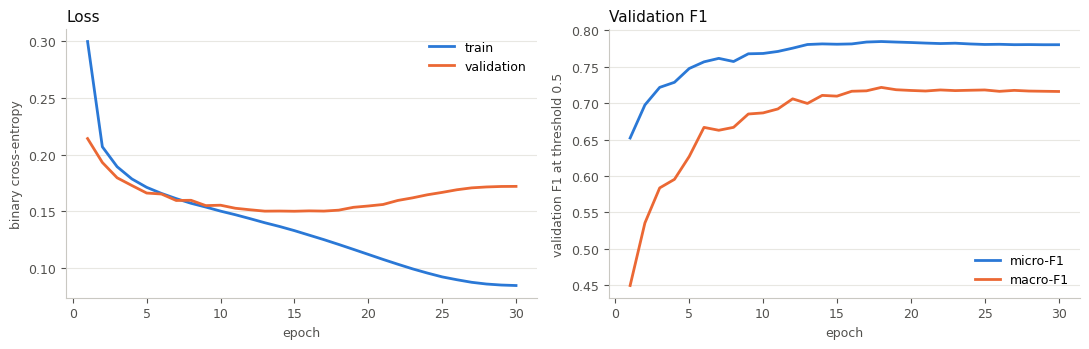
\includegraphics[width=\linewidth]{figures/curves.png}
\caption{Training and validation loss (left) and validation F1 at threshold 0.5 (right) over 30 epochs.}
\label{fig:curves}
\end{figure}

\subsection{Per-class performance}

Performance follows two things: how visually distinct a class is and how often it occurs
(Table~\ref{tab:perclass}, Figure~\ref{fig:perclass}). \emph{Marine waters} is almost solved, with an F1 of
98.2\%. \emph{Coniferous forest}, \emph{Arable land}, \emph{Inland waters} and \emph{Mixed forest} all
exceed 82\%. The weakest classes are \emph{Industrial or commercial units} (53.6\%) and \emph{Natural
grassland and sparsely vegetated areas} (54.3\%), each present in about 2\% of patches. For both, recall
is far lower than precision: the model predicts them rarely but is usually right when it does.

The two rarest classes, \emph{Beaches, dunes, sands} and \emph{Coastal wetlands}, have only 221 and 310
test patches yet reach an F1 near 60\%, higher than several more common classes. Frequency alone does
not determine difficulty. The mixed and transitional classes, \emph{Transitional woodland, shrub} and
\emph{Land principally occupied by agriculture, with significant areas of natural vegetation}, are common
but score below 70\%, which is consistent with their boundaries being hard to see in RGB.

\begin{table}[!htbp]
\centering
\caption{Per-class test results at threshold 0.5, ordered by F1. Precision, recall, F1 and average
precision (AP) in per cent.}
\label{tab:perclass}
\small
\begin{tabular}{lrrrrr}
\toprule
Class & Test patches & Precision & Recall & F1 & AP \\
\midrule
Marine waters                                   & 18,023 & 98.4 & 98.0 & 98.2 & 99.8 \\
Coniferous forest                               & 39,532 & 87.4 & 85.5 & 86.4 & 94.4 \\
Arable land                                     & 47,150 & 86.7 & 85.1 & 85.9 & 94.3 \\
Inland waters                                   & 16,177 & 90.2 & 79.2 & 84.3 & 91.8 \\
Mixed forest                                    & 42,641 & 81.5 & 83.2 & 82.3 & 90.3 \\
Agro-forestry areas                             &  7,261 & 78.1 & 78.7 & 78.4 & 88.0 \\
Urban fabric                                    & 17,928 & 81.3 & 75.4 & 78.2 & 87.5 \\
Broad-leaved forest                             & 34,130 & 82.3 & 72.1 & 76.9 & 87.2 \\
Pastures                                        & 24,170 & 78.2 & 74.5 & 76.3 & 86.4 \\
Complex cultivation patterns                    & 25,638 & 72.7 & 70.5 & 71.6 & 78.3 \\
Agriculture with natural vegetation             & 32,052 & 70.7 & 66.0 & 68.3 & 76.1 \\
Transitional woodland, shrub                    & 36,211 & 71.5 & 63.8 & 67.5 & 77.1 \\
Inland wetlands                                 &  5,349 & 77.0 & 57.2 & 65.7 & 72.7 \\
Moors, heathland and sclerophyllous vegetation  &  3,859 & 68.4 & 62.8 & 65.5 & 72.1 \\
Permanent crops                                 &  6,812 & 70.0 & 58.2 & 63.6 & 71.2 \\
Coastal wetlands                                &    310 & 64.0 & 56.1 & 59.8 & 60.9 \\
Beaches, dunes, sands                           &    221 & 56.3 & 62.4 & 59.2 & 66.1 \\
Natural grassland and sparsely vegetated areas  &  2,799 & 72.3 & 43.5 & 54.3 & 59.7 \\
Industrial or commercial units                  &  2,808 & 65.9 & 45.2 & 53.6 & 57.3 \\
\bottomrule
\end{tabular}
\end{table}

\begin{figure}[!htbp]
\centering
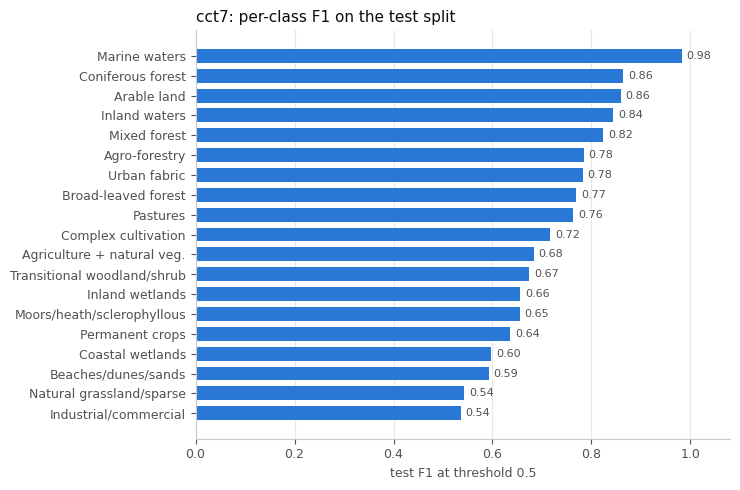
\includegraphics[width=0.78\linewidth]{figures/per_class_f1.png}
\caption{Per-class F1 on the test split at threshold 0.5.}
\label{fig:perclass}
\end{figure}

\subsection{Training cost}

The 30 epochs took 38.5 minutes in total, about 1.3 minutes per epoch including validation. The 2024
version of this study reported about 20 minutes per epoch with $32\times32$ crops and about 5 hours per
epoch on full patches. The hardware differs (a Colab TPU then, an A100 now), so this is not a controlled
comparison. Most of the difference nevertheless comes from the pipeline: the earlier code decoded every
image on every step and fed the transformer 900 tokens per patch.

\subsection{Comparison with the published benchmark}

Table~\ref{tab:compare} sets CCT-7 beside a selection of the models in~\cite{papoutsis}. Its micro-F1 of
78.4\% is higher than every benchmark row reproduced in the 2024 version of this study, the best of which
was VGG19 at 77.7\%, and is 0.6 points below the benchmark's best F-score of 79.0\% (WRN-B5-ECA).

\begin{table}[!htbp]
\centering
\caption{CCT-7 beside selected models from Papoutsis et al.~\cite{papoutsis}. All scores in per cent.
The benchmark models use multispectral input and a larger patch set, so the rows are not directly
comparable (see text). A dash marks a value not available.}
\label{tab:compare}
\small
\begin{tabular}{@{}llrrrrr@{}}
\toprule
Model & Source & Parameters & Accuracy & Precision & Recall & F1 \\
\midrule
\textbf{CCT-7} & \textbf{This study, RGB} & \textbf{3.9\,M} & \textbf{64.5} & \textbf{80.8} & \textbf{76.1} & \textbf{78.4} \\
\midrule
WRN-B5-ECA    & \cite{papoutsis} & 5.2\,M  & --   & 82.0 & 76.1 & 79.0 \\
WRN-B4-ECA    & \cite{papoutsis} & 1.0\,M  & --   & 82.4 & 75.5 & 78.8 \\
VGG19         & \cite{papoutsis} & 20\,M   & 63.6 & 81.7 & 74.2 & 77.7 \\
ViTM/20       & \cite{papoutsis} & 9\,M    & 62.7 & 80.6 & 73.8 & 77.1 \\
ResNet50      & \cite{papoutsis} & 23\,M   & 62.4 & 78.8 & 75.0 & 76.8 \\
DenseNet121   & \cite{papoutsis} & 7\,M    & 62.3 & 79.2 & 74.5 & 76.8 \\
ViT/20        & \cite{papoutsis} & 7\,M    & 62.1 & 80.5 & 73.1 & 76.6 \\
WRN-B0-ECA    & \cite{papoutsis} & 0.3\,M  & 61.7 & 81.5 & 71.8 & 76.3 \\
EfficientNetB0-ECA & \cite{papoutsis} & 3\,M & 61.4 & 79.6 & 72.9 & 76.1 \\
MLPMixer      & \cite{papoutsis} & 0.4\,M  & 60.3 & 79.1 & 71.8 & 75.2 \\
K-Branch CNN  & \cite{papoutsis} & 36\,M   & 47.3 & 63.4 & 65.1 & 64.2 \\
\midrule
CCT-2, 2024 (mis-scored) & Sect.~\ref{sec:revisit} & 0.4\,M & -- & 25.1 & 13.5 & 17.6 \\
\bottomrule
\end{tabular}
\end{table}

This comparison is indicative, not like-for-like, for three reasons:

\begin{itemize}
  \item \textbf{Input.} The benchmark models were trained on the Sentinel-2 spectral bands, excluding
        only bands 1, 9 and 10. This study uses three 8-bit RGB channels. Near-infrared and short-wave
        infrared bands carry much of the signal for vegetation and water, so the RGB model works with
        less information.
  \item \textbf{Patches.} The benchmark used the full archive of about 590,000 patches. This study uses
        the 519,284 patches that remain after snow- and cloud-affected patches are removed, which is
        likely an easier set.
  \item \textbf{Procedure.} Optimiser, schedule and augmentation differ, and the result here is from one
        run with one random seed.
\end{itemize}

The first point works against CCT-7 and the second in its favour. What the table supports is that CCT-7
performs in the same range as established architectures with several times as many parameters.

%------------------------------------------------------------------------------
\section{Revisiting the 2024 Study}
\label{sec:revisit}

The 2024 version of this study trained CCT-2 and CCT-4 and reported precision of about 25\%, recall of
about 14\% and micro-F1 of about 18\% for both. It concluded that CCTs were not viable for BigEarthNet
under limited computing resources. A review of that code found six problems
(Table~\ref{tab:problems}). The first one alone invalidates the reported scores.

\begin{table}[!htbp]
\centering
\caption{Problems in the 2024 pipeline and how this revision addresses them.}
\label{tab:problems}
\small
\begin{tabularx}{\linewidth}{@{}r L L L@{}}
\toprule
 & Problem & Effect & Correction \\
\midrule
1 & The test set was shuffled before prediction, and the predictions were then scored against labels in
    their original order.
  & Precision, recall and F1 compared each prediction with the labels of a different image.
  & One ordered pass in which predictions and labels come from the same batch. \\
\addlinespace
2 & ``Accuracy'' was categorical accuracy: whether the single highest-scoring class is among the true
    labels.
  & Not a multi-label metric and not the accuracy of~\cite{papoutsis}. It also selected the checkpoint.
  & Micro-Jaccard accuracy; checkpoint selected by validation micro-F1. \\
\addlinespace
3 & Training on random $32\times32$ crops of $120\times120$ patches.
  & The model saw 7\% of each patch but was asked for the labels of the whole patch.
  & Full patches; flips and $90^{\circ}$ rotations only. \\
\addlinespace
4 & Images decoded on every step; 900 tokens per full patch.
  & About 5 hours per epoch on full patches, which forced the crop and a 4-epoch run.
  & Data decoded once and held on the GPU; 225 tokens. \\
\addlinespace
5 & A stray quotation mark in the checkpoint path.
  & The best weights were not the ones evaluated.
  & The best checkpoint is reloaded before testing. \\
\addlinespace
6 & Label smoothing of 0.1 on 19 independent binary outputs; constant learning rate.
  & Smaller effects on calibration and convergence.
  & No label smoothing; warm-up and cosine decay. \\
\bottomrule
\end{tabularx}
\end{table}

\paragraph{Evidence for the evaluation error.}
When predictions are compared with the labels of unrelated images, the precision for a class equals the
fraction of images that carry that class, whatever the model has learned. The 2024 per-class precision
values match the class frequencies with a correlation of 0.999. That pattern is the signature of
predictions scored at chance.

\paragraph{Control experiment.}
To confirm this, the error was reproduced deliberately on the CCT-7 trained here. Its test predictions
were randomly permuted and scored against the labels in their original order
(Table~\ref{tab:control}). Micro-F1 falls from 78.4\% to 24.5\%, and the correlation between per-class
precision and class frequency is 1.000.

\begin{table}[!htbp]
\centering
\caption{Effect of misaligned evaluation on the same CCT-7 predictions, with the 2024 results for
reference. All values in per cent.}
\label{tab:control}
\begin{tabular}{lrrr}
\toprule
Evaluation & Precision & Recall & Micro-F1 \\
\midrule
CCT-7, aligned (correct)                 & 80.8 & 76.1 & 78.4 \\
CCT-7, labels shuffled (control)         & 25.3 & 23.8 & 24.5 \\
\midrule
2024: CCT-2, $32\times32$ crops, 30 epochs   & 25.1 & 13.5 & 17.6 \\
2024: CCT-4, $32\times32$ crops, 30 epochs   & 24.8 & 14.1 & 18.0 \\
2024: CCT-2, full patches, 4 epochs          & 26.0 & 22.8 & 24.3 \\
\bottomrule
\end{tabular}
\end{table}

The 2024 full-patch result (precision 26.0\%, recall 22.8\%, F1 24.3\%) is almost identical to what a
well-trained model scores under shuffled labels. This suggests that the 2024 full-patch CCT-2 may have
been learning the task, and that its improvement over the cropped models reflected a higher rate of
positive predictions more than a real gain in measured skill. The 2024 models were never scored correctly,
so their true performance is unknown.

%------------------------------------------------------------------------------
\section{Discussion}

The corrected benchmark reverses the conclusion of the 2024 study. A CCT with under four million
parameters learns BigEarthNet-19 from RGB alone to a micro-F1 of 78.4\%, and does so in well under an hour
on a single GPU. Neither accuracy nor cost is an obstacle to using CCTs for land cover classification.

The 2024 study did identify one real problem. Random cropping is unsuitable for a multi-label dataset
whose labels describe the whole patch, and removing it was the right change. The study also attributed
the long training time to the model, whereas it came from the data pipeline and the sequence length.
Adding one convolutional block to the tokenizer reduced the sequence from 900 to 225 tokens, in line with
Hassani et al.'s own approach to larger inputs.

Class imbalance remains the main limit on performance. Micro-F1 exceeds macro-F1 by six points, and the
gap comes from a handful of rare classes with low recall. Per-class thresholds recover only part of it.
The overfitting visible after epoch 15 also suggests that stronger regularisation or augmentation could
help.

More broadly, the 2024 result shows how an evaluation error can pass for a negative finding. Scores far
below every published baseline were explained by the model and the dataset, when a comparison of per-class
precision with class frequency, or a check that the model could fit a single batch, would have exposed
the problem.

%------------------------------------------------------------------------------
\section{Limitations and Future Work}

\begin{itemize}
  \item \textbf{One model, one run.} Only CCT-7 was trained, with a single seed. CCT-2 and CCT-4, the
        models of the 2024 study, have not yet been re-run with the corrected pipeline, so the effect of
        model size is not measured and no confidence interval can be given.
  \item \textbf{No baseline under identical conditions.} No convolutional model has been trained with the
        same data and procedure. Until one is, the comparison with~\cite{papoutsis} is indicative only.
        The pipeline includes a ResNet-18 configuration for this purpose.
  \item \textbf{RGB input.} Training on the multispectral bands would allow a direct comparison with the
        published benchmark and would probably improve the vegetation classes.
  \item \textbf{Imbalance.} Class-weighted or focal losses and resampling were not tested.
  \item \textbf{Dataset version.} BigEarthNet version~2 updates the labels and the splits.
        Results on it would be more current.
\end{itemize}

%------------------------------------------------------------------------------
\section{Conclusion}

This study set out to determine whether Compact Convolutional Transformers are viable for land cover
classification on BigEarthNet. With a corrected training and evaluation pipeline, CCT-7 reaches a test
micro-F1 of 78.4\% and a macro-F1 of 72.4\% using 3.94 million parameters and 38.5 minutes of training on
one GPU. The poor results reported in 2024 were caused by scoring predictions against the wrong labels,
which a control experiment reproduces. CCTs are a viable and inexpensive option for this task. Training
the smaller variants and a convolutional baseline under the same conditions is the next step.

%------------------------------------------------------------------------------
\section*{Acknowledgements}

I would like to thank my supervisor, Dr.\ Songnian Li, for his patience and support, and my second
reader, Dr.\ Ceni Babaoglu, for her kindness and help throughout the original project.

\section*{Code Availability}

The training and evaluation notebook, \texttt{CCT\_BigEarthNet\_v2.ipynb}, the per-class results and the
original 2024 code are available at
\url{https://github.com/Wgullett/Benching-Compact-Convolutional-Transformers-with-BigEarthNet}.

%------------------------------------------------------------------------------
\begin{thebibliography}{99}

\bibitem{papoutsis} I. Papoutsis, N. I. Bountos, A. Zavras, D. Michail, and C. Tryfonopoulos,
``Benchmarking and scaling of deep learning models for land cover image classification,''
\emph{ISPRS Journal of Photogrammetry and Remote Sensing}, vol.~195, pp.~250--268, Jan.~2023.
doi:10.1016/j.isprsjprs.2022.11.012

\bibitem{hassani} A. Hassani \emph{et al.}, ``Escaping the big data paradigm with compact transformers,''
arXiv:2104.05704, 2021.

\bibitem{zhao} Z. Zhao, T. Chen, and J. Li, ``Compact convolutional transformer for landslide
susceptibility mapping,'' in \emph{IGARSS 2023 -- IEEE International Geoscience and Remote Sensing
Symposium}, Jul.~2023. doi:10.1109/igarss52108.2023.10281512

\bibitem{bokhari} S. A. Bokhari \emph{et al.}, ``Assessing land cover transformation for urban
environmental sustainability through satellite sensing,'' \emph{Sustainability}, vol.~14, no.~5, p.~2810,
Feb.~2022. doi:10.3390/su14052810

\bibitem{urbanelli} A. Urbanelli, L. Barco, E. Arnaudo, and C. Rossi, ``A multimodal supervised machine
learning approach for satellite-based wildfire identification in Europe,'' in \emph{IGARSS 2023 -- IEEE
International Geoscience and Remote Sensing Symposium}, Jul.~2023. doi:10.1109/igarss52108.2023.10282227

\bibitem{choudhary} S. Choudhary and K. R. Ramkumar, ``A detailed analysis of artificial intelligence
support to measure negative impacts created by the abnormal growth of Prosopis juliflora: A review,'' in
\emph{3rd International Conference on Intelligent Sustainable Systems (ICISS)}, Dec.~2020.
doi:10.1109/iciss49785.2020.9315978

\bibitem{kim} M. Kim, D. Kim, and G. Kim, ``Examining the relationship between land use/land cover (LULC)
and land surface temperature (LST) using explainable artificial intelligence (XAI) models: A case study of
Seoul, South Korea,'' \emph{International Journal of Environmental Research and Public Health}, vol.~19,
no.~23, 15926, 2022. \url{https://www.mdpi.com/1660-4601/19/23/15926}

\bibitem{vincent} M. J. Vincent, P. Varalakshmi, U. Nithya, S. Sona, and A. M. Thomas, ``Land use land
cover change detection using semi-automatic classification: A case study in Chennai, Tiruvallur and
Kanchipuram districts,'' in \emph{International Conference on Data Science, Agents \& Artificial
Intelligence (ICDSAAI)}, Dec.~2022. doi:10.1109/icdsaai55433.2022.10028962

\bibitem{shaik} R. U. Shaik \emph{et al.}, ``Exploring canopy temperature and height dynamics in forest
ecosystems,'' in \emph{IEEE International Conference on Metrology for eXtended Reality, Artificial
Intelligence and Neural Engineering (MetroXRAINE)}, Oct.~2023. doi:10.1109/metroxraine58569.2023.10405767

\bibitem{mannan} A. Mannan \emph{et al.}, ``Application of land-use/land cover changes in monitoring and
projecting forest biomass carbon loss in Pakistan,'' \emph{Global Ecology and Conservation}, vol.~17,
Jan.~2019. doi:10.1016/j.gecco.2019.e00535

\bibitem{naushad} R. Naushad, T. Kaur, and E. Ghaderpour, ``Deep transfer learning for land use and land
cover classification: A comparative study,'' \emph{Sensors}, vol.~21, no.~23, p.~8083, Dec.~2021.
doi:10.3390/s21238083

\bibitem{jamali} A. Jamali, S. K. Roy, D. Hong, P. M. Atkinson, and P. Ghamisi, ``Spatial-gated multilayer
perceptron for land use and land cover mapping,'' \emph{IEEE Geoscience and Remote Sensing Letters},
vol.~21, pp.~1--5, 2024. doi:10.1109/lgrs.2024.3354175

\bibitem{kunwar} S. Kunwar and J. Ferdush, ``Mapping of land use and land cover (LULC) using EuroSAT and
transfer learning,'' arXiv:2401.02424, 2024.

\bibitem{islam} Md.~F. Islam \emph{et al.}, ``Identifying hurricane damage using explainable compact
transformer with convolutional embedding,'' in \emph{25th International Conference on Computer and
Information Technology (ICCIT)}, Dec.~2022. doi:10.1109/iccit57492.2022.10054917

\bibitem{sumbul} G. Sumbul, M. Charfuelan, B. Demir, and V. Markl, ``BigEarthNet: A large-scale benchmark
archive for remote sensing image understanding,'' in \emph{IGARSS 2019 -- IEEE International Geoscience
and Remote Sensing Symposium}, Jul.~2019. doi:10.1109/igarss.2019.8900532

\end{thebibliography}

\end{document}
